%To compile as handout, use
%pdflatex "\def\ishandout{1} \input{filename.tex}"
%Defaults to non-handout mode (with slide reveals)
\ifdefined\ishandout
  \documentclass[handout]{beamer}
\else
  \documentclass{beamer}
\fi
 
\usepackage{econ103slides} 

\date{Optional Addendum to Lecture 23}


\begin{document} 




%%%%%%%%%%%%%%%%%%%%%%%%%%%%%%%%%%%%%%%%

\begin{frame}[plain]
	\titlepage 
	

\end{frame} 

%%%%%%%%%%%%%%%%%%%%%%%%%%%%%%%%%%%%%%%%
\begin{frame}
\frametitle{Example of Calculating Power: Is this coin fair?}

\begin{block}
{Flip a Possibly Unfair Coin $n$ Times}
$X_1, \hdots, X_n \sim \mbox{iid Bernoulli}(p)$ where $p$ may not equal 1/2
\end{block}

\begin{block}
	{Test $H_0\colon p = 0.5$ against $H_1\colon p \neq 0.5$}
	Under $H_0$ and if $n$ is large the CLT gives 
	$$\displaystyle T_n = \frac{\widehat{p} - 0.5}{\sqrt{\frac{0.5(1-0.5)}{n}}}\approx N(0,1)$$
\end{block}

\begin{alertblock}
	{The Idea Behind Statistical Power}
	How does the test statistic behave if the  $H_0$ is \emph{false}? What is the sampling distribution of $T_n$ \emph{under the alternative}: $H_1\colon p\neq 0.5$
\end{alertblock}

\end{frame}
%%%%%%%%%%%%%%%%%%%%%%%%%%%%%%%%%%%%%%%%
\begin{frame}
% \frametitle{Sampling Dist.\ of $T_n$ Under the Alternative $H_1\colon p \neq 0.5$}

\begin{block}
	{Key Distributional Result}
	Center and standardize $\widehat{p}$ using \emph{true} $p \implies$ standard normal:
	$$Z = \frac{\widehat{p} - p}{\sqrt{\frac{p(1-p)}{n}}}  \approx N(0,1)$$
\end{block}

\begin{block}
	{Under the Alternative $p\neq 0.5$}
	$T_n$ is \emph{incorrectly centered and scaled}: $\displaystyle T_n = \frac{\widehat{p} - 0.5}{\sqrt{\frac{0.5(1-0.5)}{n}}} \neq N(0,1)$
\end{block}

\begin{alertblock}
	{How We'll Proceed}
	Use algebra to express $T_n$ in terms of $Z$, which we know is $N(0,1)$, and constants. This will give the distribution of $T_n$ under $H_1$.
\end{alertblock}
\end{frame}
%%%%%%%%%%%%%%%%%%%%%%%%%%%%%%%%%%%%%%%%
\begin{frame}
\frametitle{This is Just Algebra}
\small
	\begin{eqnarray*}
	T_n &=&\frac{\widehat{p} - 0.5}{\sqrt{\frac{0.5(1-0.5)}{n}}} =\sqrt{n}(2\widehat{p} - 1)\\ \\
	&=& \sqrt{n} \left[2\widehat{p} -1 + (2p -2p)\right] = \sqrt{n}\left[ 2\left(\widehat{p} - p\right) + 2p -1\right]\\ \\
	&=& \sqrt{n}\left[ 2\left(\widehat{p} - p\right) \left(\frac{\sqrt{p(1-p)/n}}{\sqrt{p(1-p)/n}}\right) + 2p -1\right]\\ \\
		&=& \sqrt{n}\left[ 2\sqrt{\frac{p(1-p)}{n}} \alert{\left(\frac{\widehat{p} - p}{\sqrt{p(1-p)/n}}\right)} + 2p -1\right]\\ \\
		&=& \left[2\sqrt{p(1-p)}\right] \alert{Z} + \sqrt{n}(2p -1)\\
		&=& a\, \alert{Z} + b
\end{eqnarray*}
\end{frame}
%%%%%%%%%%%%%%%%%%%%%%%%%%%%%%%%%%%%%%%%
\begin{frame}
\frametitle{Distribution of Test Statistic Under $H_1\colon p \neq 0.5$ }

From the previous slide,
	$$T_n =\frac{\widehat{p} - 0.5}{\sqrt{\frac{0.5(1-0.5)}{n}}} = \alert{a Z + b}$$
where:
	\begin{eqnarray*}
		Z &=& \frac{\widehat{p} - p}{\sqrt{p(1-p)/n}} \approx N(0,1)\\ 
		a &=& 2\sqrt{p(1-p)}\\ 
		b &=& \sqrt{n}(2p -1) 
	\end{eqnarray*}

\vspace{1em}
\alert{Hence: $T_n \approx N(\mu = b, \sigma^2 = a^2)$}
\end{frame}
%%%%%%%%%%%%%%%%%%%%%%%%%%%%%%%%%%%%%%%%
\begin{frame}[c]\frametitle{Distribution of $T_n$ Under the Alternative}
    
    $$\boxed{T_n =\frac{\widehat{p} - 0.5}{\sqrt{\frac{0.5(1-0.5)}{n}}} \approx N\left(\sqrt{n}(2p-1), 4p(1-p) \right)}$$

\begin{block}
	{Note That:}
	\begin{enumerate}
		\item Mean depends on $p$ and $n$
		\item Variance depends only on $p$
		\item If $p=0.5$ so $H_0$ is true, this reduces to a standard normal:
		\begin{eqnarray*}
		\mbox{Mean} &=&  \sqrt{n}(2p-1) = \sqrt{n}(2\times 1/2 - 1) = 0\\
			\mbox{Variance} &=& 4p(1-p) = 4 \times 1/2 \times (1 - 1/2) = 1\\
		\end{eqnarray*}
	\end{enumerate}
\end{block}

\end{frame}

%%%%%%%%%%%%%%%%%%%%%%%%%%%%%%%%%%%%%%%%
\begin{frame}
	\frametitle{\href{http://glimmer.rstudio.com/fditraglia/power_proptest/}{http://glimmer.rstudio.com/fditraglia/power\_proptest/}}
\framesubtitle{Ignore everything except the solid curve and play around with the first two sliders.}

\begin{figure}
	\fbox{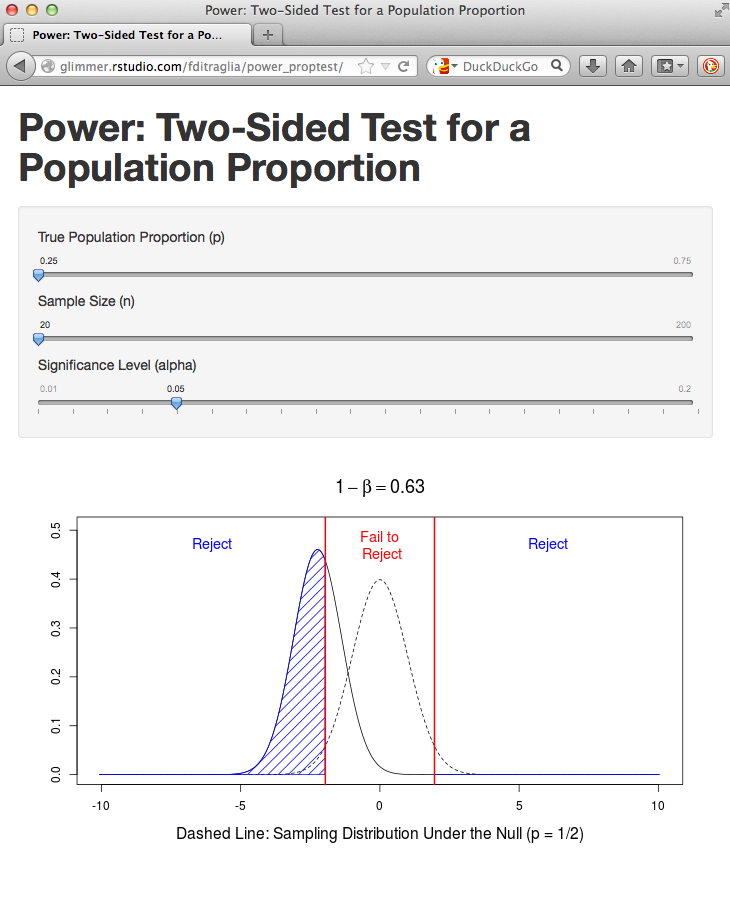
\includegraphics[scale = 0.22]{./images/power_proptest_screenshot}}
\end{figure}

\end{frame}
%%%%%%%%%%%%%%%%%%%%%%%%%%%%%%%%%%%%%%%%
\begin{frame}
\frametitle{Now We can Calculate Power!}
\small
\begin{block}{Decision Rule for Two-sided Test}
Reject $H_0\colon p = 0.5$ provided that $\alert{|T_n| \geq \texttt{qnorm}(1 - \alpha/2)}$
\end{block}

\begin{block}{If the null is false (i.e.\ under $H_1\colon p \neq 0.5$)}
	$$T_n = \frac{\widehat{p} - 0.5}{\sqrt{\frac{0.5(1-0.5)}{n}}} \approx N\left(\sqrt{n}(2p-1), 4 p(1-p)  \right)$$
\end{block}
\begin{block}{Thus, the probability of rejecting a false null is:}
	$$\boxed{\mbox{Power}(\alpha, p, n) = P\left( |Y| \geq c\right)  = P(Y \leq -c) + P(Y\geq c)}$$
		\begin{eqnarray*}
			 c &=&\texttt{qnorm}(1 - \alpha/2) \\
			 Y &\sim& N\left(\sqrt{n}(2p-1), 4 p(1-p)  \right)
		 \end{eqnarray*} 
\end{block}
\end{frame}
%%%%%%%%%%%%%%%%%%%%%%%%%%%%%%%%%%%%%%%%
\begin{frame}
	\frametitle{\href{http://glimmer.rstudio.com/fditraglia/power_proptest/}{http://glimmer.rstudio.com/fditraglia/power\_proptest/}}
\framesubtitle{Now look at everything and try changing all the sliders!}

\begin{figure}
	\fbox{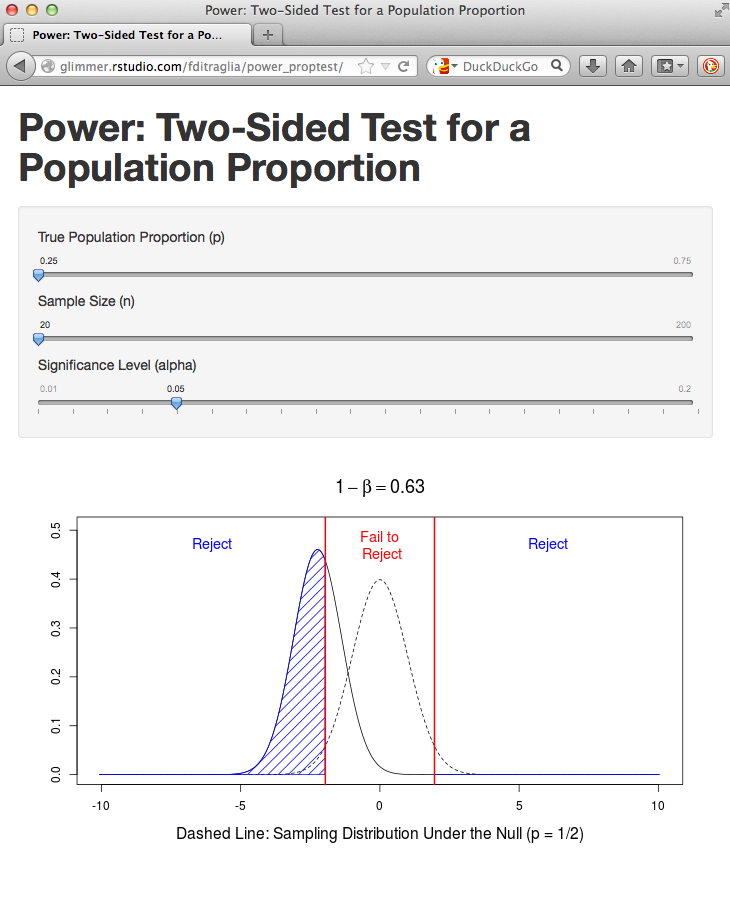
\includegraphics[scale = 0.22]{./images/power_proptest_screenshot}}
\end{figure}

\end{frame}
%%%%%%%%%%%%%%%%%%%%%%%%%%%%%%%%%%%%%%%%\begin{frame}
\begin{frame}
\begin{center}
	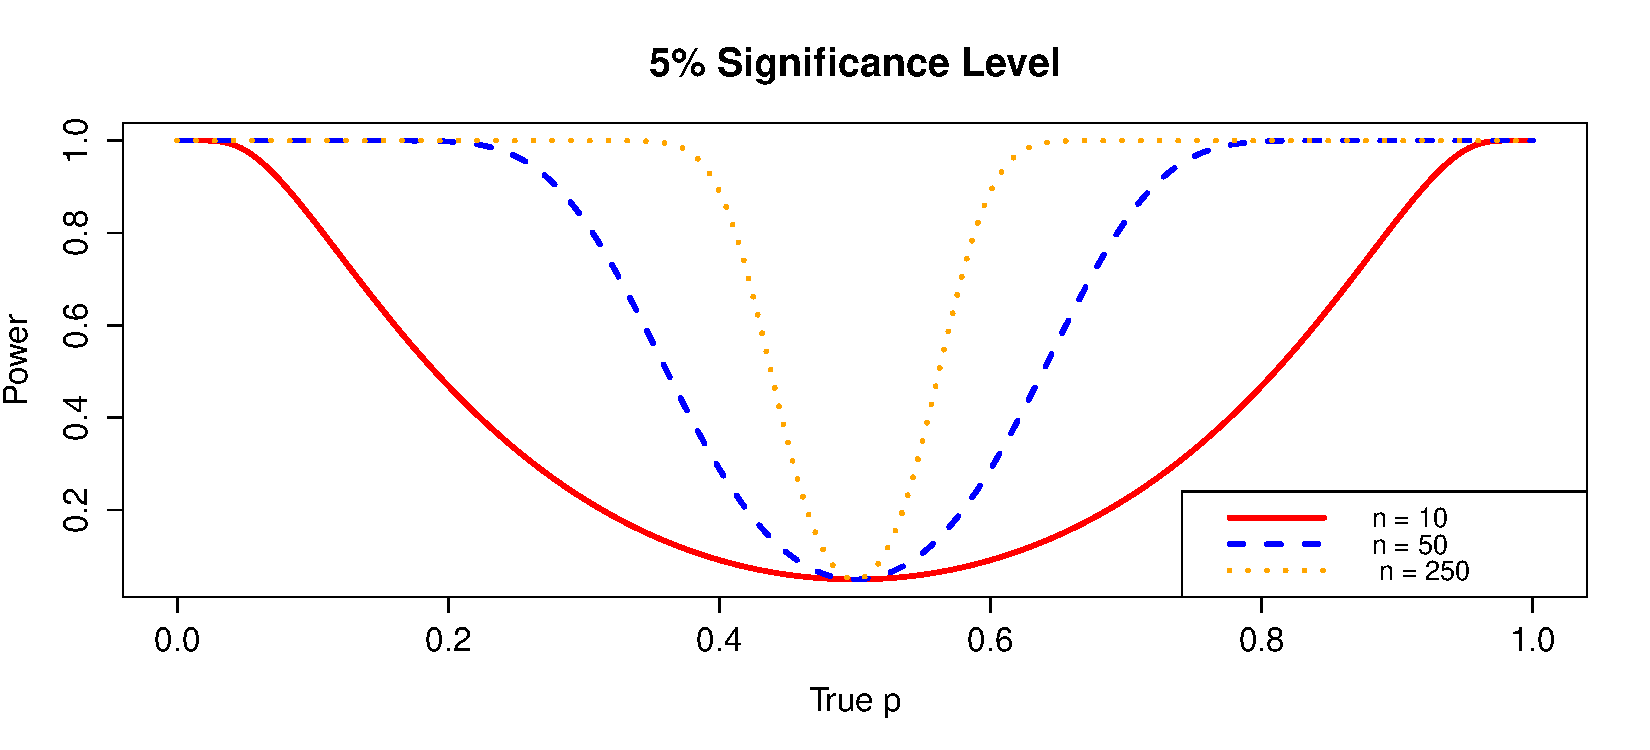
\includegraphics[scale=0.37]{./images/power_change_n}\\
	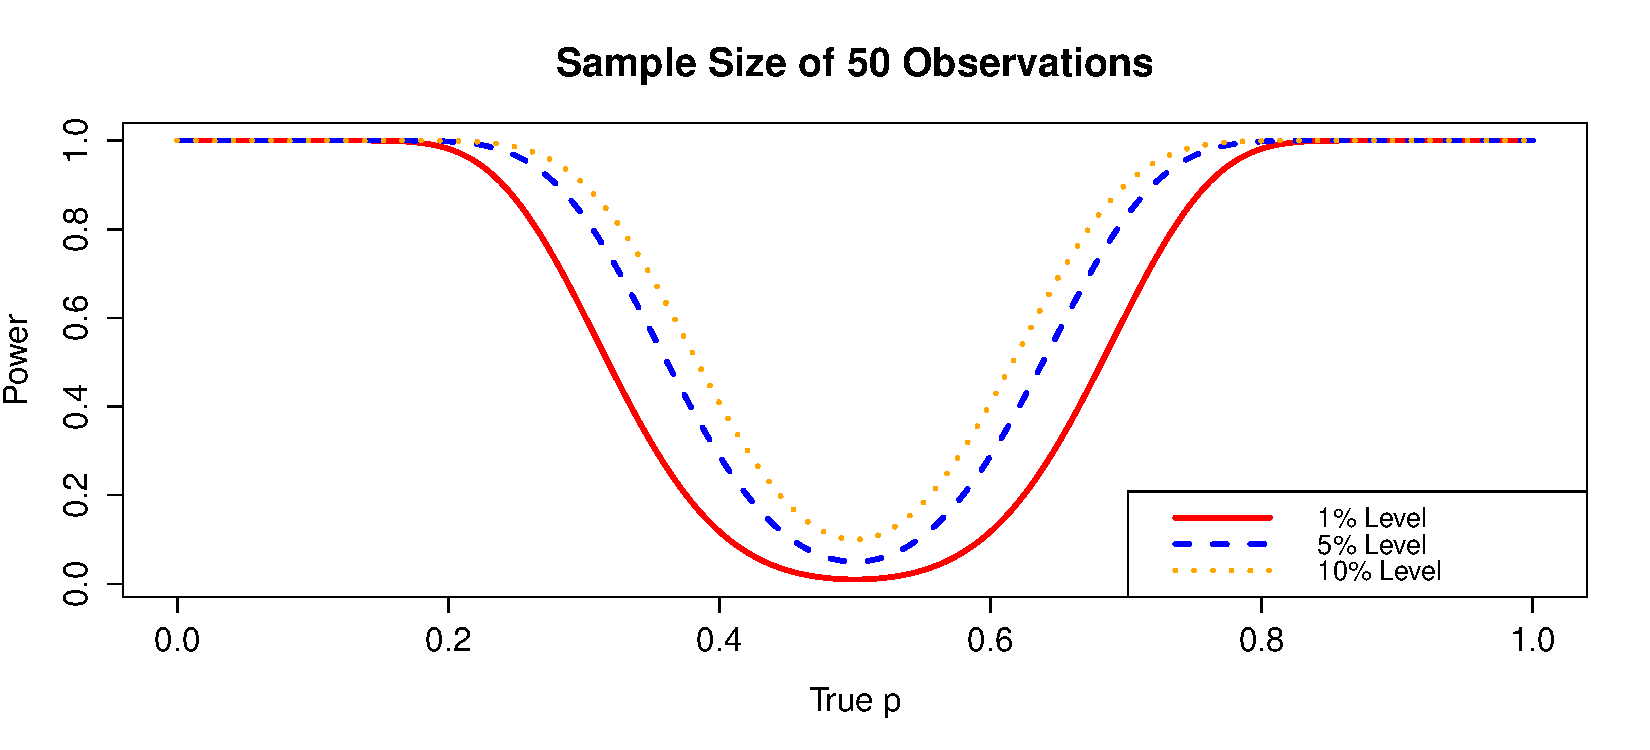
\includegraphics[scale=0.37]{./images/power_change_a}
\end{center}
\end{frame}
%%%%%%%%%%%%%%%%%%%%%%%%%%%%%%%%%%%%%%%%
\begin{frame}
\frametitle{Some Intuition about Power for the Coin Example}
\small
	\begin{itemize}
	\item Equals prob.\ of rejecting false null, i.e.\ convicting a guilty person.
	\item Tells us how large a sample we would need to detect a given discrepancy from ``fairness'' of the coin: $p = 0.5$
		\begin{itemize}
			\item Small deviations from $p=0.5$ unlikely to be detected unless the sample size is large.
			\item Large deviations from $p=0.5$ very likely to be detected even if the sample size is small.
		\end{itemize}
		\item For a \emph{given} degree of ``unfairness'' (deviation from $p = 0.5$)
			\begin{itemize}
				\item Higher significance level ($\alpha$) $\implies$ higher power ($1-\beta$)
				\item Large sample size ($n$) $\implies$ higher power ($1-\beta$)
			\end{itemize}
	\end{itemize}
\end{frame}

%%%%%%%%%%%%%%%%%%%%%%%%%%%%%%%%%%%%%%%%

\begin{frame}
\frametitle{An Important Point}
For any discrepancy from $p = 0.5$, there is always a sample size large enough to make the power of our test \emph{arbitrarily close to one}. In other words, we can be almost certain to detect an effect, no matter how small, provided that we use a large enough sample. \alert{However, this does not mean that the affect we have found is important}.

\vspace{2em}
If it turned out that the true probability of heads was closer to 0.50001 rather than 0.5, should we really care? 
\end{frame}
% %%%%%%%%%%%%%%%%%%%%%%%%%%%%%%%%%%%%%%%%
\begin{frame}[fragile]
\frametitle{An R Function to Calculate Power For Coin Example}
\footnotesize
	\begin{eqnarray*}
		\mbox{Power}(\alpha, p, n) &=& P\left(Y \leq -c\right) + P\left(Y\geq c\right)\\
			 c &=&\texttt{qnorm}(1 - \alpha/2) \\
			 Y &\sim& N\left(\sqrt{n}(2p-1), 4 p(1-p)  \right)
		 \end{eqnarray*} 

\begin{verbatim}
coin.power <- function(a, p, n){
    c <-  qnorm(1 - a/2)	
    mu <- sqrt(n) * (2 * p - 1) 	
    sigma <- sqrt(4 * p * (1 - p))
    
    less.than <- pnorm(-c, mean = mu, sd = sigma)
    greater.than <- 1 - pnorm(c, mean = mu, sd = sigma)
    power <- less.than + greater.than
    return(power)
}
\end{verbatim}
\end{frame}


%%%%%%%%%%%%%%%%%%%%%%%%%%%%%%%%%%%%%%%%

\begin{frame}[fragile]
\frametitle{Here's Some Code for You to Play Around With}
\footnotesize
You can use the function \texttt{coin.power} to calculate power for specific values of $p, n,$ and $\alpha$
\begin{verbatim}
coin.power(a = 0.05, p = 0.55, n = 100)
coin.power(a = 0.05, p = 0.55, n = 1000)
coin.power(a = 0.1, p = 0.55, n = 100)
coin.power(a = 0.05, p = 0.6, n = 100)
\end{verbatim}
or to make plots similar to those on slide 28
\begin{verbatim}
alternatives <- seq(from = 0, to = 1, by = 0.001)
power <- coin.power(a = 0.05, alternatives, n = 10)
plot(alternatives, power, xlab = `True p', ylab = `Power', type = `l')
\end{verbatim}
Try out different choices for $p,n$ and $\alpha$ and see what you get! I'll post this R code to save typing.

\end{frame}
%%%%%%%%%%%%%%%%%%%%%%%%%%%%%%%%%%%%%%%%
\end{document}